% Sample document for SBGames papers
% Uses a slightly modified IEEE VGTC template in conference mode

\documentclass{vgtc}                          % final (conference style)

%% These three lines bring in essential packages: ``mathptmx'' for Type 1 
%% typefaces, ``graphicx'' for inclusion of EPS figures. and ``times''
%% for proper handling of the times font family.

\usepackage{mathptmx}
\usepackage{graphicx}
\usepackage{times}
\usepackage{xspace}
\usepackage{url}
\usepackage{verbatim}

\usepackage{listings}
\usepackage{color}
    \definecolor{light}{gray}{0.97}
    \definecolor{dark}{gray}{0.30}
\lstset{
%columns=fullflexible,
%basicstyle=\ttfamily,
escapeinside={||},
    %mathescape=true,
    language=C, % choose the language of the code
    basicstyle=\fontfamily{pcr}\selectfont\scriptsize\color{black},
    keywordstyle=\color{black}\bfseries, % style for keywords
    numbers=none, % where to put the line-numbers
    numberstyle=\tiny, % the size of the fonts that are used for the line-numbers
    backgroundcolor=\color{light},
    showspaces=false, % show spaces adding particular underscores
    showstringspaces=false, % underline spaces within strings
    showtabs=false, % show tabs within strings adding particular underscores
    %frame=single, % adds a frame around the code
    tabsize=2, % sets default tabsize to 2 spaces
    %rulesepcolor=\color{gray}
    captionpos=b, % sets the caption-position to bottom
    breaklines=false, % sets automatic line breaking
    %breakatwhitespace=false,
    numbersep=2em,
    % C was used in the blocksworld example to refer to block C and nowhere else
    emph={par,or,hor,do,end,loop,await,emit,input,event,call,with,%
          var,and,then,else,return,pure,deterministic,nohold,finalize,%
          class, every, FOREVER, this, spawn, in, pool, watching, until, 
          interface, each, abort, when, signal, PROC, CHAN, SIGNAL, PAR, not,
          bool, data, tag, escape, new, traverse,implementation,output,
          native,@const,@pure,@safe,define},
    emphstyle={\bfseries},
    commentstyle=\color{dark}\scriptsize,
    %xleftmargin=20pt,
    %xrightmargin=20pt,
    framesep=20pt,
    %upquote=true,
    %aboveskip={1.5\baselineskip},
}

\newcommand{\CEU}{\textsc{C\'{e}u}\xspace}
\newcommand{\code}[1] {{\small{\texttt{#1}}}}
\newcommand{\ax}{\code{[a]}\xspace}
\newcommand{\bx}{\code{[b]}\xspace}

%% We encourage the use of mathptmx for consistent usage of times font
%% throughout the proceedings. However, if you encounter conflicts
%% with other math-related packages, you may want to disable it.

%% If you are submitting a paper to a conference for review with a double
%% blind reviewing process, please replace the value ``0'' below with your
%% OnlineID. Otherwise, you may safely leave it at ``0''.
\onlineid{0}

%% declare the category of your paper, only shown in review mode
\vgtccategory{Research}

%% Paper title.

\title{Structured Synchronous Reactive Programming for Game Development
        \\ \Large{Case Study: On Rewriting Pingus from C++ to \CEU}}

\author{Francisco Sant'Anna
        \\ Departamento de Inform\'atica e Ci\^encia da Computa\c{c}\~ao, UERJ
        \\ francisco@ime.uerj.br}

\abstract{Abstract.

\smallskip

\noindent \textbf{Keywords:} Radiosity, global illumination, constant time.
}

%% Copyright space is enabled by default as required by guidelines.
%% It is disabled by the 'review' option or via the following command:
% \nocopyrightspace

\begin{document}

\firstsection{Introduction}

\maketitle

Pingus%
\footnote{Pingus: \url{http://pingus.seul.org/}}
is an open-source clone of Lemmings%
\footnote{Lemmings: \url{https://en.wikipedia.org/wiki/Lemmings_(video_game)}},
a puzzle-platformer video game.      
The objective of the game is to guide a group of penguins through a number of
obstacles towards a designated exit%
\footnote{Pingus gameplay: \url{https://www.youtube.com/watch?v=MKrJgIFtJX0}}.

\begin{figure}
\centering
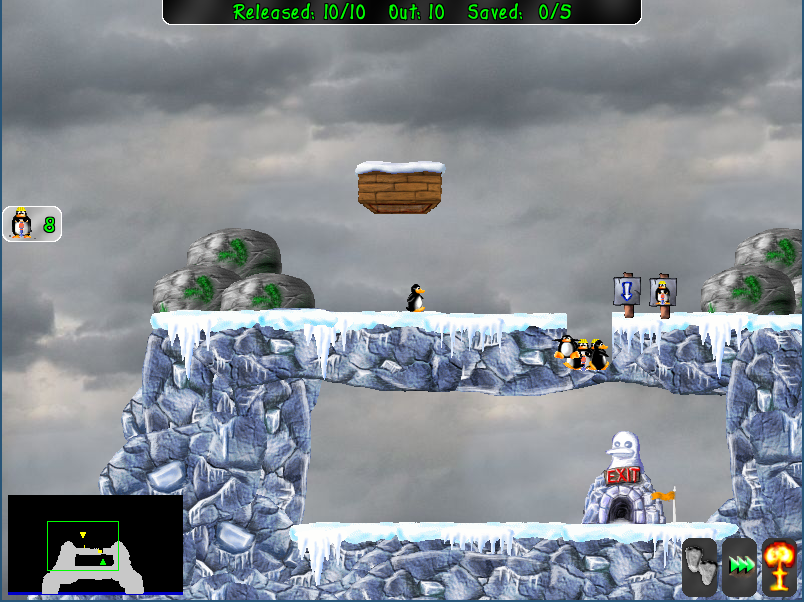
\includegraphics[width=\columnwidth]{pingus}
\caption{Pingus gameplay.
\label{fig.sweeney}
}
\end{figure}

Pingus is developed in standard object-oriented C++, the \emph{lingua franca}
of game development \cite{games.patterns}.
The codebase is about 40.000 lines of code (LoCs)%
\footnote{Pingus repository: \url{https://github.com/Pingus/pingus/tree/7b255840c201d028fd6b19a2185ccf7df3a2cd6e/src}}, divided into
the engine, level editor, auxiliary libraries, and the game logic itself.

According to Tim Sweeney (of Unreal Engine fame), about half the complexity in
game development resides in \emph{simulation} (aka \emph{game logic}), but
which accounts for only 10\% of the CPU budget~\cite{games.sweeney}.
The game logic ``models the state of the game world as interacting objects
evolve over time''.
The high development costs contrasting with the low impact on performance
appeals for alternatives with productivity in mind, especially considering that
it is the game logic that varies the most between projects.
Sweeney states that ``will gladly sacrifice 10\% of our performance for 10\%
higher productivity''.

\begin{figure}
\centering
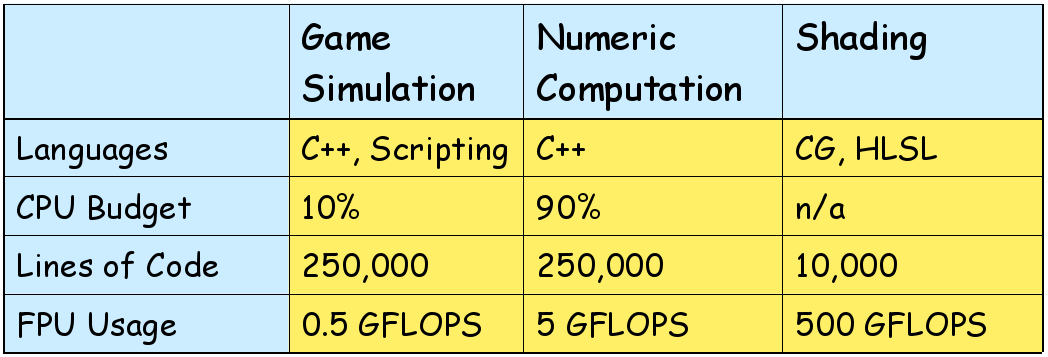
\includegraphics[width=\columnwidth]{sweeney}
\caption{Three kinds of code~\cite{games.sweeney}.
\label{fig.sweeney}
}
\end{figure}

Object-oriented games use the \emph{observer pattern}~\cite{games.patterns}
in the game logic to handle events from the environment (e.g., key presses and
timers) and also as a notification mechanism between game entities.
%
The observers are short-lived callbacks which must execute as fast as possible
and in real time to keep the game reactive to incoming events.
%
For this reason, callbacks cannot contain long-lasting locals and loops, which
are elementary capabilities of classical structured
programming~\cite{rp.deprecating,rp.rescala,sync_async.cooperative}.
%
In this sense, callbacks actually disrupt structured programming, becoming
``our generation's \code{goto}''.%
\footnote{``Callbacks as our Generations' Go To Statement'':
\url{http://tirania.org/blog/archive/2013/Aug-15.html}}%
\footnote{``Escape from Callback Hell'':
\url{http://elm-lang.org/learn/Escape-from-Callback-Hell.elm}}

\CEU~\cite{ceu.sensys13,ceu.mod15} is a programming language that aims to offer
a concurrent and expressive alternative to C/C++ with the characteristics that
follow:
%
\begin{itemize}
\item \emph{Reactive}: code only executes in reactions to events.
\item \emph{Structured}: programs use structured control mechanisms, such as
      \code{await} (to suspend a line of execution), and \code{par} (to combine
      multiple lines of execution).
\item \emph{Synchronous}: reactions run atomically and to completion on each
      line of execution, i.e., there's no implicit preemption or real
      parallelism.
\end{itemize}
%
Structured reactive programming eliminates callbacks, letting programmers write
code in direct and sequential style and recover from the inversion of control
imposed by the observer pattern~\cite{rp.deprecating}.
%
\CEU supports logical parallelism with a resource-efficient implementation in
terms of memory and CPU usage~\cite{ceu.sensys13}.
The runtime is single threaded and the language requires no garbage
collection.

Contributions:
    - patterns
    - solutions

\section{Control-Flow Patterns}

The rewriting process consisted of identifying sets of callbacks implementing
*control-flow behaviors* in the game and translating them to \CEU using
appropriate structured constructs.
As an example, a double mouse click is characterized by a first click, followed
by a maximum amount of time, followed by a second click.
This behavior depends on different events (clicks and timers) which have to
occur in a particular order.
In C++, the implementation involves callbacks crossing reactions to successive
events which manipulate state variables explicitly.

We can identify control-flow behaviors in C++ by looking for class members with
identifiers resembling verbs, statuses, and counters (e.g.,
\code{pressed},
\code{particle\_thrown},
\code{mode}, and
\code{delay\_count}).
Good chances are that variables with these ``suspicious names'' encode some
form of control-flow progression that cross multiple callback invocations.

We selected 9 representative game behaviors and describe their
implementations in C++ and \CEU.
We also categorized these examples in 5 abstract C++ control-flow patterns that
likely apply to other games:

\begin{enumerate}
\item \emph{Finite State Machines}:
    State machines describe the behavior of entities by mapping event
    occurrences to transitions between states that trigger appropriate actions.
\item \emph{Continuation Passing}:
    The completion of a long-lasting activity may carry a continuation, i.e.,
    some action to execute next.
\item \emph{Dispatching Hierarchies}:
    Entities typically form a dispatching hierarchy in which a container that
    receives a stimulus automatically forwards it to its managed children.
\item \emph{Lifespan Hierarchies}:
    Entities typically form a lifespan hierarchy in which a terminating
    container entity automatically destroys its managed children.
\item \emph{Signaling Mechanisms}:
    Entities often need to communicate explicitly through signaling mechanisms,
    especially if there is no hierarchy relationship between them.
\end{enumerate}

\subsection{Finite State Machines \\ Case Study: The Armageddon Button Double Click}
%\label{sec.patterns.fsm}

State machines describe the behavior of entities by mapping event occurrences
to transitions between states that trigger appropriate actions.

%\subsection{The Armageddon Button Double Click}
%\label{sec.patterns.fsm.armageddon}

\begin{figure}
\centering
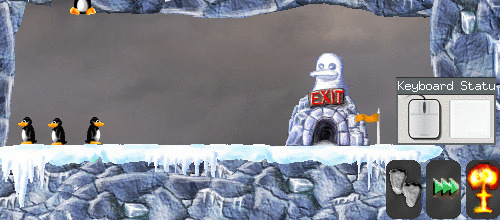
\includegraphics[width=\columnwidth]{double-click-opt}
\caption{Double click detection.
\label{fig.armageddon}
}
\end{figure}

In Pingus, a double click in the \emph{Armageddon} button at the bottom right
of the screen literally explodes all pingus (Figure~\ref{fig.armageddon}).
Figure~\ref{fig.armageddon.code} compares the implementations in C++ and \CEU.

\begin{figure*}
\begin{minipage}[t]{0.55\linewidth}
\begin{lstlisting}[numbers=left,xleftmargin=3em]
ArmageddonButton::ArmageddonButton(<...>):
    RectComponent(<...>),
    pressed(false); // button initially not pressed
    press_time(0);    // how long since 1st click?
    <...>
{
    <...>
}

void ArmageddonButton::draw (<...>) {
    <...>
}

void ArmageddonButton::update (float delta) {
    <...>
    if (pressed) {
        press_time += delta;
        if (press_time > 1.0f) {
            pressed = false; // give up, 1st click
            press_time = 0;  // was too long ago
        }
    } else {
        <...>
        press_time = 0;
    }
}

void ArmageddonButton::on_click (<...>) {
    if (pressed) {
        server->send_armageddon_event();
    } else {
        pressed = true;
    }
}
\end{lstlisting}
\centering\small{\ax Implementation in C++}
\end{minipage}
%
\begin{minipage}[t]{0.45\linewidth}
\begin{lstlisting}[numbers=left,xleftmargin=3em]
do
    var& RectComponent c = <...>;
    <...>
    loop do
        await c.component.on_click;
        watching 1s do
            await c.component.on_click;
            break;
        end
    end
    <...>
    emit outer.game.go_armageddon;
end




















.
\end{lstlisting}
\centering\small{\bx Implementation in \CEU}
\end{minipage}
%\rule{8.4cm}{0.37pt}
\caption{ Shared-memory concurrency in \CEU:
example \ax is safe because the trails access \code{x} atomically in different 
reactions;
example \bx is unsafe because both trails access \code{y} in the same reaction.
\label{lst.shared}
}
\end{figure*}

In C++, the class \code{ArmageddonButton} implements methods for rendering the
button and handling mouse and timer events.
The listing focus on the double click detection, hiding unrelated parts with
\code{<...>}.
%
The methods \code{update} (ln. 14--26) and \code{on\_click} (ln. 28--34) are
examples of \emph{short-lived callbacks}, which are pieces of code that execute
atomically in reaction to external input events.
The callback \code{on\_click} reacts to mouse clicks detected by the button
base class \code{RectComponent} (ln. 2), while the callback \code{update}
continuously reacts to the passage of time, frame by frame.
Callbacks are short lived because they must react to input as fast as possible
to let other callbacks execute, keeping the game with real-time responsiveness.
%
The class first initializes the variable \code{pressed} to track the first
click (ln. 3,32).
It also initializes the variable \code{press\_time} to count the time since the
first click (ln. 4, 17).
If another click occurs within 1 second, the class signals the double click to
the application (ln. 30).
Otherwise, the \code{pressed} and \code{press\_time} state variables are reset
(ln. 19--20). 
%
Figure~\ref{fig.armageddon.fsm} illustrates how we can model the double-click 
behavior in C++ as a state machine.
The circles represent the state of the variables in the class, while the arrows 
represent the callbacks manipulating state.
%
Note in the code how the accesses to the state variables are spread
across the entire class.
For instance, the distance between the initialization of \code{pressed} (ln.
3) and the last access to it (ln. 32) is over 40 lines in the original file.
Arguably, this dispersion of code across methods makes the understanding and 
maintenance of the double-click behavior more difficult.
Also, even though the state variables are private, unrelated methods such as 
\code{draw}`, which is defined in middle of the class (ln. 10--12), can
potentially access them.

\begin{figure}
\centering
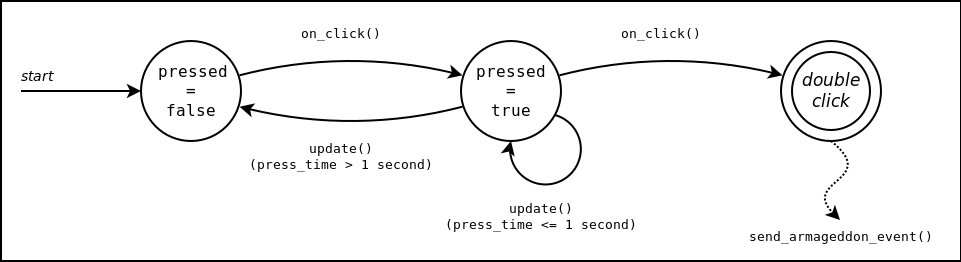
\includegraphics[width=\columnwidth]{double-click}
\caption{State machine for the \emph{Armageddon} double click.
\label{fig.armageddon.fsm}
}
\end{figure}

\CEU provides structured constructs to deal with events, aiming to eradicate
explicit manipulation of state variables for control-flow purposes.
%
The loop detection (ln. 4--10) awaits the first click (ln. 5) and then, while
watching 1 second (ln. 6--9), awaits the second click (ln. 7).
If the second click occurs within 1 second, the \code{break} terminates the
loop (ln. 8) and the \code{emit} signals the double click to the application
(ln. 12).
Otherwise, the \code{watching} block as a whole aborts and restarts the loop, 
falling back to the first click \code{await} (ln. 5).
%
Double click detection in \CEU doesn't require state variables and is entirely
self-contained in the \code{loop} body (ln. 4--10).
Furthermore, these 7 lines of code \emph{only} detect the double click, leaving
the actual effect to happen outside the loop (ln. 12).

\subsection{Continuation Passing \\ Case Study: Advancing Pages in the Story Screen}

The completion of a long-lasting activity may carry a continuation, i.e., some
action to execute next.

\begin{figure}
\centering
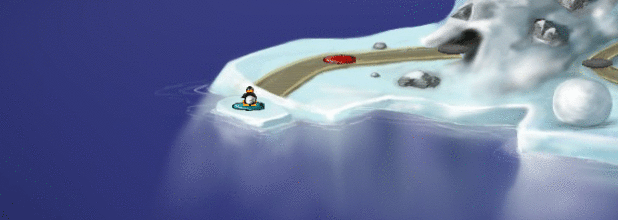
\includegraphics[width=\columnwidth]{story-anim}
\caption{The Story screen.
\label{fig.story}
}
\end{figure}

The clickable \emph{blue dots} in the campaign world map transit to ambience
story screens (Figure~\ref{fig.story}).
A story is composed of multiple pages and, inside each page, the words of the
story appear incrementally over time.
A first click in the button \code{>>>} fast forwards the words to show the full 
page.
A second click advances to the next page, until the story terminates.
If the page completes before a click (due to the time elapsing), a first click 
advances to the next page.

\begin{figure*}
\begin{minipage}[t]{0.55\linewidth}
\begin{lstlisting}[numbers=left,xleftmargin=3em]
StoryScreenComponent::StoryScreenComponent (<...>) :
    <...>
{
    pages        = <...>; // vector with loaded pages
    current_page = pages.back(); // first loaded page
    displayed    = false; // if current is complete
    <...>
}

<...>   // draw page over time

void StoryScreenComponent::update (<...>) {
    <...>
    if (&lt;all-words-appearing&gt;) {
        displayed = true;
    }
}

void StoryScreenComponent::next_text() {
    if (!displayed) {
        displayed = true;
        <...>     // remove current page
    } else {
        pages.pop_back();
        if (!pages.empty()) { // next page
            current_page = pages.back();
            displayed    = false;
            <...>
        } else {
            <...> // terminates the story screen
        }
    }
}
\end{lstlisting}
\centering\small{\ax Implementation in C++}
\end{minipage}
%
\begin{minipage}[t]{0.45\linewidth}
\begin{lstlisting}[numbers=left,xleftmargin=3em]
code/await Story (void) -> bool do
    <...>
    event void next_text; // clicks in >>>

    { pages = <...>; } // same as in C++
    loop i in [0 <- {pages.size()}[ do
        par/or do
            watching next_text do
                <...> // advance text
            end
            await next_text;
        with
            <...> // redraw _pages[i]
        end
    end
end

















.
\end{lstlisting}
\centering\small{\bx Implementation in \CEU}
\end{minipage}
%\rule{8.4cm}{0.37pt}
\caption{ Shared-memory concurrency in \CEU:
example \ax is safe because the trails access \code{x} atomically in different 
reactions;
example \bx is unsafe because both trails access \code{y} in the same reaction.
\label{lst.shared}
}
\end{figure*}

\begin{figure}
\centering
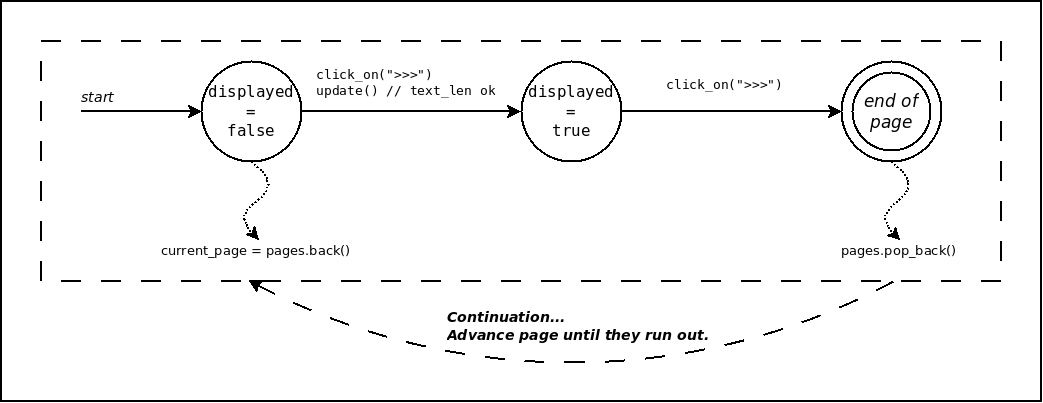
\includegraphics[width=\columnwidth]{story}
\caption{State machine for the Story screen.
\label{fig.story}
}
\end{figure}

In C++, the class \code{StoryScreenComponent} implements the method
\code{next\_text}, which is a callback for clicks in \code{>>>}.
%
The variable `pages` (ln. 4--5, 24--26) is a vector holding each page, but
which also encodes \emph{continuations} for the story progress:
each call to \code{next\_text} that advances the story (ln. 23--32) removes the 
current page (ln. 24) and sets the next action to perform (i.e., ``display a
new page'') in the variable \code{current\_page} (ln. 26).
Figure~\ref{fig.story} illustrates the continuation mechanism to advance 
pages and also a state machine for fast forwarding words (inside the dashed
rectangle).
The state variable \code{displayed} (ln. 6,15,20,21,27) switches between the
behaviors ``advancing text'' and ``advancing pages'', which are both handled
intermixed inside the method \code{next\_text}.

The code in \CEU uses the internal event \code{next\_text}, which is emitted
from clicks in \code{>>>}.
%
The sequential navigation from page to page uses a loop in direct style
(ln. 6--15) instead of explicit state variables for the continuation and state
machine.
While the text advances in an inner loop (hidden in ln. 9), we watch the
\code{next\_text} event that fast forwards it.
The loop may also eventually terminate with the time elapsing normally.
This way, we do not need a variable (such as `displayed` in C++) to switch 
between the states ``advancing text'' and ``advancing pages''.
The \code{par/or} makes the page advance logic to execute in parallel with the
redrawing code (ln. 13).
Whenever the page advances, the redrawing code is automatically aborted
(due to the \code{or} modifier).
The \code{await next\_text} in sequence (ln. 11) is the condition to advance to
the next page.
%
Note that, unlike the implementation in C++, the ``advancing text'' behavior is
not intermixed with the ``advancing pages'' behavior, instead, it is
encapsulated inside the inner loop nested with a deeper indentation (ln. 9).

\bibliographystyle{abbrv}
\bibliography{my,other}
\end{document}
